% !TEX root = ../main.tex
\section{Evaluation}
\label{sec:eval}

\subsection{Experimental Setup}
\textbf{Algorithm.} We evaluate Open-Sora v1.2 STDiT3-XL/2~\cite{zheng2024opensora} on VBench~\cite{huang2024vbench}. All quality runs generate 64-frame, $512\times512$ videos with 30 rectified-flow steps under identical prompts and sampling settings. We compare Original (FP16), ViDiT-Q~\cite{zhao2025viditq} (linear-only W8A8), TeaCache~\cite{liu2025teacache} (FP16 timestep caching), and Q-DARE (QAC with W8A8 linear and attention execution).

\textbf{Hardware.} We compare against ViDA~\cite{ding2025vida} and NVIDIA A100~\cite{nvidiaA100}. Q-DARE is synthesized in TSMC 28\,nm at 1\,GHz and normalized to 7\,nm with DeepScaleTool~\cite{sarangi2021deepscaletool}, following ViDA's comparison setting. A cycle-level simulator models accelerator latency. A100 is measured on the same 64-, 256-, and 512-frame, $512\times512$ Open-Sora workloads; Q-DARE uses ViDA's 1\,GHz and 256\,GB/s off-chip-bandwidth setting.

\subsection{Algorithm Quality}
\begin{figure}[t]
  \centering
  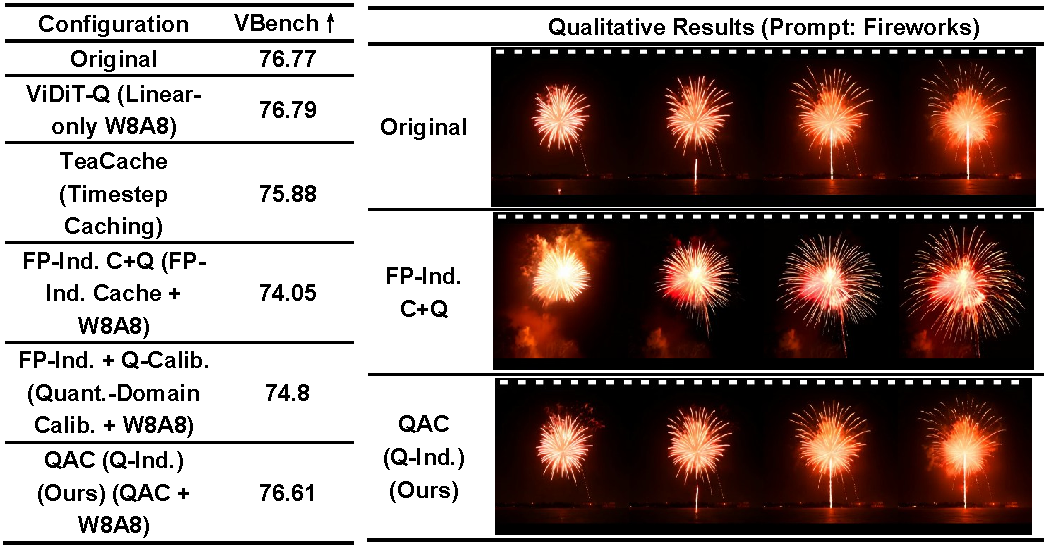
\includegraphics[width=\columnwidth]{fig/gen_img.pdf}
  \caption{Open-Sora v1.2 quality comparison under identical prompts and sampling settings.}
  \label{fig:quality}
\end{figure}

Fig.~\ref{fig:quality} shows that Q-DARE reaches 76.61 VBench, only 0.16 below FP16 (76.77), while jointly applying timestep caching and W8A8 linear/attention execution. TeaCache reaches 75.88 under FP16 caching, whereas ViDiT-Q reaches 76.79 with quantization alone. Q-DARE therefore retains near-FP16 generation quality while combining both acceleration dimensions.

\subsection{Hardware Evaluation}
\textbf{Comparison with ViDA.}
Table~\ref{tab:vida_comparison} summarizes the implementation characteristics and comparison with ViDA~\cite{ding2025vida}. Q-DARE reaches \QDAREViDAThroughputGeo$\times$ geomean video throughput and \QDAREViDAreaGeo$\times$ geomean area efficiency. Its throughput advantage increases from 1.007$\times$ at 64 frames to 1.091$\times$ at 512 frames, showing that the adaptive dataflows extend beyond the representative short-$T$ case used to explain the microarchitecture.

\begin{table}[t]
\centering
\caption{Implementation and normalized comparison with ViDA.}
\label{tab:vida_comparison}
\scriptsize
\setlength{\tabcolsep}{3.0pt}
\renewcommand{\arraystretch}{1.04}
\resizebox{\columnwidth}{!}{%
\begin{tabular}{@{}ccc@{}}
\toprule
\textbf{Metric} & \textbf{Q-DARE} & \textbf{ViDA~\cite{ding2025vida}} \\
\midrule
\multicolumn{3}{c}{\textbf{Implementation Characteristics}} \\
\midrule
Technology & 28$\rightarrow$7 nm & 32$\rightarrow$7 nm \\
Frequency & 1.0\,GHz & 1.0\,GHz \\
Precision & INT8/FP16 & FP16 \\
\multirow{2}{*}{Compute Units}
  & 1296 INT8 MACs & \multirow{2}{*}{640 FP16 MACs} \\
  & 36 FP16 MACs & \\
On-chip SRAM & 238.5\,KB & N/R \\
Memory BW & 256\,GB/s & 256\,GB/s \\
Area (mm$^2$) & 0.134 & 2.03 \\
Power (mW) & 43.6 & N/R \\
\midrule
\multicolumn{3}{c}{\textbf{Normalized Results}} \\
\midrule
64F Throughput & 1.007$\times$ & 1.00$\times$ \\
256F Throughput & 1.071$\times$ & 1.00$\times$ \\
512F Throughput & 1.091$\times$ & 1.00$\times$ \\
Throughput Geomean & \textbf{\QDAREViDAThroughputGeo$\times$} & 1.00$\times$ \\
Area Eff. Geomean & \textbf{\QDAREViDAreaGeo$\times$} & 1.00$\times$ \\
\bottomrule
\end{tabular}%
}
\vspace{1pt}
\parbox{\columnwidth}{\scriptsize
64F, 256F, and 512F denote video frames; all workloads use $512\times512$ resolution. Throughput and area efficiency are normalized to ViDA.}
\end{table}

\textbf{Comparison with A100.}
Fig.~\ref{fig:a100_comparison} compares STDiT step throughput and energy efficiency with A100. Q-DARE provides 10.02--11.88$\times$ step-throughput speedup across the three video lengths, with a \QDAREStepGeoA$\times$ geomean. Energy-efficiency gains range from 365.8$\times$ to 381.6$\times$, with a \QDAREEnergyGeoA$\times$ geomean. The stable gain across video lengths indicates that adaptive-control overhead remains small as temporal length grows; the step-throughput metric isolates accelerator speed from the additional reduction in executed steps due to caching.

\begin{figure}[t]
  \centering
  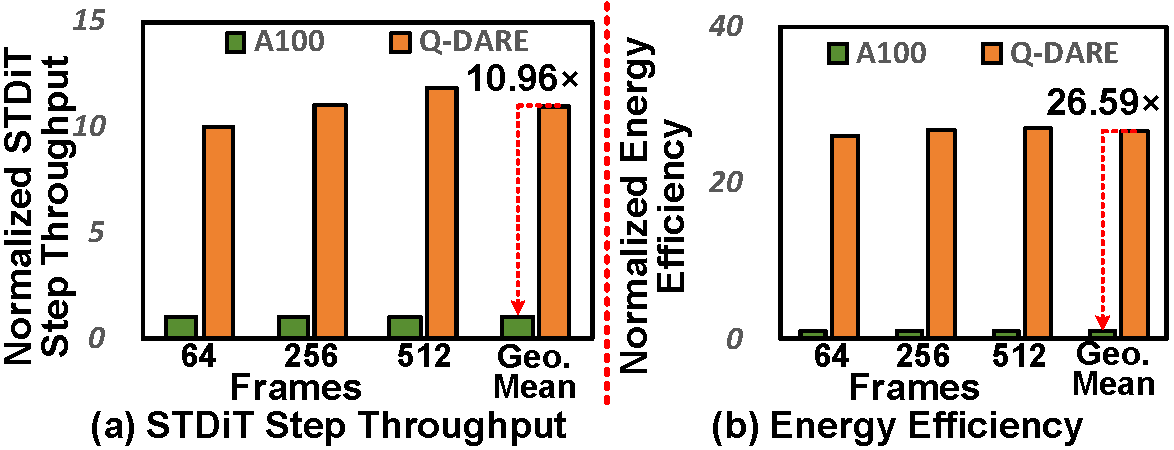
\includegraphics[width=\columnwidth]{fig/vs_A100.pdf}
  \caption{A100 comparison across video lengths: (a) STDiT step throughput and (b) energy efficiency.}
  \label{fig:a100_comparison}
\end{figure}

Overall, the results separate the two sources of gain: QAC removes redundant STDiT executions, while DARE improves utilization of each executed step. The near-FP16 VBench score shows that combining these two mechanisms does not introduce a corresponding quality collapse.
